\documentclass{article}
\usepackage[utf8]{inputenc}
\usepackage{fullpage}
\usepackage{tikz}
\usepackage{pgfplots}
\usepackage{amsfonts}
\usepackage{graphics}
\title{Simulation Numérique de l'amortissement Landau dans les plasmas}
\date{2019}
\author{Yassine MOUFTAH\\Guillaume ROUMAGE}
\begin{document}
\maketitle
\newpage
\tableofcontents
\newpage
\noindent Dans tout le document, les problèmes seront étudiés sur un intervalle de temps noté $[0;T]$, avec $T \in ]0; + \infty[$. Pour discrétiser le problème afin de faire des simulations numériques, on choisit un nombre de pas $N$. L'intervalle $[0;T]$ est subdivisé en $N$ sous-intervalles. Le pas de temps, représenté par $dt$, est alors donné par la formule : $dt = \frac{T}{N}$.\\
Les situations en 1D seront étudiés sur un segment de longueur $L$.\\
Les champs électriques étudiés seront dans la grande majorité du temps discrétisé en un nombre $I$ de points. Le pas d'espace, représenté pat $dx$, ets alors donné par la formule : $dx = \frac{L}{I}$.
\newpage
\section{Introduction}
\section{Plasma : définition, intérêts scientifiques et industriels}
Il est courant de dire que la matière possède trois états : l'état solide, l'état liquide, ainsi que l'état gazeux. Mais en réalité, il existe un quatrième état de la matière : c'est le plasma.\\
Comme nous le savons, les atomes sont composés d'un noyau, contenant des protons et des neutrons, autour duquel gravitent des électrons. A l'état solide, liquide ou gazeux, les électrons qui orbitent autour des atomes restent sur leurs orbites. Lorsque de la matière est chauffé, elle passe successivement de l'état solide à l'état liquide, puis de l'état liquide à l'état gazeux. Lorsque le gaz est chauffé à très haute température (supérieure à $10^4$ K), une partie de ce gaz devient un plasma.\\
Cette haute température libèrent les électrons des l'orbites de l'atome auquel ils étaient rattaché, qui peuvent désormais se déplacer dans le gaz. Celui-ci devient alors un mélange d'électrons et d'ions positifs.\\
\\
L'analyse numérique permet de reproduire par le calcul une réalité physique. Cette simulation peut être effectuée pour plusieurs raisons : l'expérience peut-être irréalisable, avoir un coût trop élevé, ou encore pour prévoir grâce aux ordinateurs comment l'expérience va se dérouler, avant de faire cette même expérience en laboratoire, en conditions réelles.\\
L'analyse numérique permet aussi de vérifier l'exactitude des modèles théoriques sous-jacents, et dégager le modèle qui peut modéliser au mieux les phénomènes physiques observés. Le schéma numérique lui-même doit être bien adapté au modèle. C'est pour cela qu'il y a différent types de méthodes numérique.
\section{Description des modèles théoriques utilisés}
\section{Description des méthodes numériques utilisés}
\section{Travail réalisé}
\subsection{Notations et constantes}
\begin{itemize}
\item Valeur d'une charge élémentaire : $e = 1.6021766208.10^{-19} C$.
\item Charge élémentaire d'un électron : $q_e = -e = -1.6021766208.10^{-19} C$.
\item Masse d'un électron : $m_e = 9.109.10^{-31} kg$.
\end{itemize}
\subsection{Simulation de mouvements de particules en 1D}
Nous simulons en premier lieu le mouvement d'une, puis de plusieurs particules en une dimension, c'est-à-dire sur un segment défini. Nous noterons cette longueur $L$. Lors de la simulation, si la particule atteint le bord droit du segment, elle est envoyée sur le bord gauche, et inversement. Cela permet à la particule de rester dans l'intervale d'espace étudié. Les particules étudiées seront les électrons. En effet, les mouvements des ions sont négligeables devant ceux des électrons. Nous considérerons donc les ions comme fixes.
\subsubsection{Avec un champs électrique nul}
Les équations donnant la position et la vitesse des électrons sont données par les systèmes suivants. Tout d'abord, en faisant l'hypothèse que le champs électrique auquel est soumis l'électron est nul.
$$
\left \{
   \begin{array}{l l l}
      x'(t)  & = & v(t) \\
      v'(t)  & = & 0 \\
	\end{array}
\right.
$$
avec $t \in [0;T]$.\\
En discrétisant et en utilisant la méthode d'Euler explicite, cela se réécrit :
$$
\left \{
   \begin{array}{l l l}
      x_{n+1}  & = & x_n + h.v_n \\
      v_{n+1}  & = & v_n \\
	\end{array}
\right.
$$
avec $n \in \{0,...,N-1\}$.\\
La vitesse étant constante, l'utilisation de la méthode d'euler symplectique n'apporte pas de préçisions supplémentaires.\\
\begin{center}
\includegraphics[scale=0.7]{mouvement_1D_sans_champs_electrique.png}
\end{center}
On remarque que dès que l'on simule plus de 100 particules, l'affichage devient lent. C'est pour cela que parfois, nous ne travaillerons qu'avec l'espace des phases des particules (le graphique de la vitesse en fonction de la position pour chaque particules). D'une part, le mouvement des particules est mieux représentés, et d'autre part, les calculs sont plus rapides.
\subsubsection{Avec un champs électrique stationnaire}
Ajoutons maintenant un champ électrique stationnaire, c'est-à-dire qui ne dépend pas du temps. Les équations décrivant la position et la vitesse des électrons sont données par :
$$
\left \{
   \begin{array}{l l l}
      x'(t)  & = & v(t) \\
      v'(t)  & = & -\frac{q_e}{m_e}.E_0(x(t)) \\
	\end{array}
\right.
$$
avec $t \in [0;T]$, $m_e$ la masse d'un électron, $q_e$ la valeur de la charge élémentaire de l'électron, $E_0$ la fonction représentant la valeur du champ électrique en fonction de la position.\\
Dans la simulation, la fonction $E_0$ utilisée est $E_0 : x \mapsto \sin(\frac{2 . \pi}{L} \times x) \times \frac{-m_e}{q_e}$.\\
\begin{center}
\includegraphics[scale=0.7]{representation_E0.png}
\end{center}
Le terme $\sin$ de $E_0$ permet d'avoir une fonction périodique sur l'intervalle de temps étudier. La multiplication par le facteur $\frac{-m_e}{q_e} \simeq \frac{10^{-30}}{10^{-19}} \simeq 10^{-11}$ permet de diminuer la valeur du champs électrique, de façon  à ce que la simulation soit exploitable.
En discrétisant et avec la méthode d'Euler explicite :
$$
\left \{
   \begin{array}{l l l}
      x_{n+1}  & = & x_n + h.v_n \\
      v_{n+1}  & = & v_n - h.\frac{q_e}{m_e}.E_0(x_n) \\
	\end{array}
\right.
$$
Ce système étant un système hamiltonien séparé, nous pouvons aussi effectué une discrétisation en utilisant la méthode d'Euler symplectique :
$$
\left \{
   \begin{array}{l l l}
      x_{n+1}  & = & x_n + h.v_n \\
      v_{n+1}  & = & v_n - h.\frac{q_e}{m_e}.E_0(x_{n+1}) \\
	\end{array}
\right.
$$
\begin{center}
\includegraphics[scale=0.7]{comparaion_explicite_symplectique.png}
\end{center}
On remarque que la méthode d'euler symplectique est plus préçise sans devoir faire de discrétisation plus fine. Pour cette raison, nous utiliserons autant que possible la méthode d'euler symplectique.
\subsubsection{Avec un champs électrique discrétisé}
Dans les deux cas précédent, le champs électrique est donné par une fonction continue. De ce fait, on pouvait savoir la valeur du champs électrique en n'importe quelle position.\\
Chaque particules est soumises à un champs électrique. Plus préçisément, il y a deux champs électrique. Le champs électrique extérieur, et celui créé par les particules, qui est auto-consistant. Il se modifie donc à chaque pas de temps, en fonction du mouvement des électrons.\\
De ce fait il faut le calculer à chaque pas de temps, et donc le discrétisé. Cela implique que le champs électrique est une liste finie de valeurs.\\
Pour simplifier la modélisation, nous considérons qu'un seul et unique champs électrique agit.\\
\\
Le calcul de la force électrique auquelle est soumise un électron se fait donc de la façon suivante :\\
Notons $E_{elec}$ la force électrique exercée sur un électron. A un $t$ instant, l'électron se trouve à une position que nous noterons $x_0$.\\
Etant donné que le champs électrique est une liste finie de valeurs, dans la majorité des cas, nous ne connaissons pas la valeur du champs électrique au point $x_0$.\\
On a $\lfloor x_0 \rfloor \leq x_0 < \lfloor x_0 \rfloor + 1$. Nous considérons donc qu'un électron à la position $x_0$ est soumis aux champs électrique des points $\lfloor x_0 \rfloor$ et $\lfloor x_0 \rfloor + 1$, car nous connaissons la valeur du champs électrique en ces deux points (par la discrétisation du champs).\\
La dernière étape consiste a pondérer le poids de chacun de ces deux champs électrique. Plus l'électron est proche de $\lfloor x_0 \rfloor$, plus le champs électrique en ce point a de l'influence. De même pour $\lfloor x_0 \rfloor + 1$.\\
D'où au final, en prenant $\alpha = x_0 - \lfloor x_0 \rfloor$ :
$$E_{elec} = (1 - \alpha) \times E_{\lfloor x_0 \rfloor} + \alpha \times E_{\lfloor x_0 \rfloor + 1}$$
\begin{center}
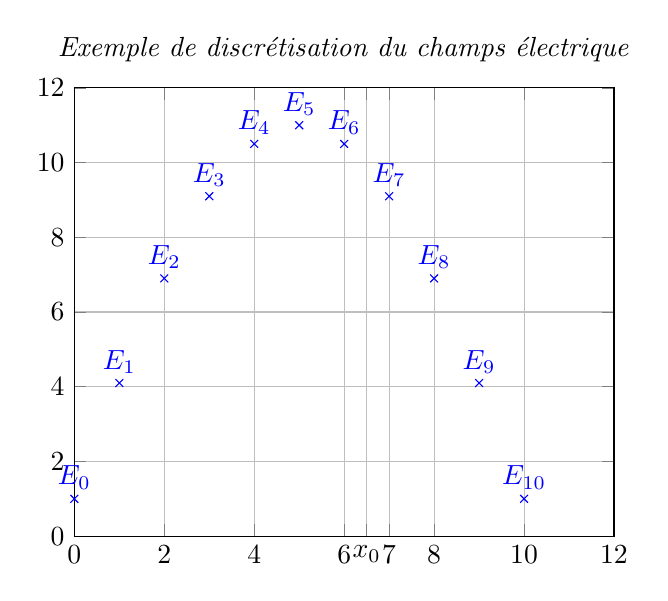
\begin{tikzpicture}
\begin{axis}[nodes near coords, point meta=explicit symbolic, grid=major, xmin=0, xmax=12, ymin=0, ymax=12, extra x ticks={6,6.5,7}, extra x tick labels={,$x_0$,7}, extra x tick style={grid=major}, title={\textit{Exemple de discrétisation du champs électrique}}]
\addplot+[only marks, mark=x] coordinates{(0,1)[$E_0$] (1,4.1)[$E_1$] (2,6.9)[$E_2$] (3,9.1)[$E_3$] (4,10.5)[$E_4$] (5,11)[$E_5$] (6,10.5)[$E_6$] (7,9.1)[$E_7$] (8,6.9)[$E_8$] (9,4.1)[$E_9$] (10,1)[$E_{10}$]};
\draw[<->] (60,40) -- (65,40);
\draw (62.5,35) node{$\alpha$};
\draw[<->] (65,40) -- (70,40);
\draw (67.5,45) node{$1 - \alpha$};
\end{axis}
\end{tikzpicture}
\end{center}
On observe qu'un électron à la position $x_0$ subira une force électrique $E_{elec} = (1 - \alpha) \times E_6 + \alpha \times E_7$.
\begin{center}
\includegraphics[scale=0.7]{discretisation_champs.png}
\end{center}
On note que plus la subdivision est fine, plus le mouvement des particules dans le champs discrétisé se rapproche du mouvement idéal, qui est celui lorsque le champs est continue.\\
Rappelons tout de même qu'étant donné qu'une méthode numérique est utilisée, bien que le mouvement se rapproche de celui voulu, il y a toujours une petite erreur d'approximation qui est introduite à chaque pas.
\subsection{Calculs relatifs aux densité}
\subsubsection{Méthode d'acceptation-rejet}
\label{sssec:acceptationRejet}
La méthode d'acceptation-rejet est une méthode permettant de simuler une loi de probabilité de densité $f$ lorsqu'il est compliqué de simuler directement cette densité. Nous expliquons ci-après le fonctionnement de la méthode d'acceptation-rejet.\\
Considérons par exemple une variable aléatoire $X$ dont la fonction de densité $f_X$ est donnée par : $f_X(x) = (x^2 + x + \frac{1}{6}) \times \mathbf{1}_{[0;1]}(x)$.
\begin{center}
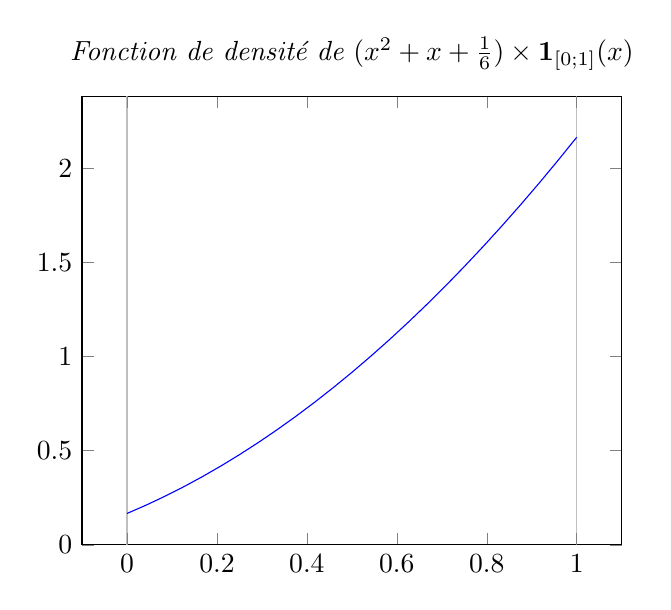
\begin{tikzpicture}
\begin{axis}[title={\textit{Fonction de densité de $(x^2 + x + \frac{1}{6}) \times \mathbf{1}_{[0;1]}(x)$}}, extra x ticks={0,1}, extra x tick labels={,}, extra x tick style={grid=major}, ymin=0]
\addplot+[mark=none] expression[domain=0:1]{x^2+x+1/6};
\end{axis}
\end{tikzpicture}
\end{center}
Le support de la loi de $X$ est de la forme $[a;b]$ avec $a,b \in \mathbb{R}$ et $a < b$. On peut donc l'inscrire dans un rectangle. Ce rectangle correspond à la densité d'une loi uniforme $u$, augmenté d'un facteur $c$. Dans notre exemple, comme la $f_X$ est définie sur $[0;1]$, on a $c = f(1)$. De manière générale, si $f_X$ est définie sur $[a;b]$, on a $c = max_{x \in [a;b]} f_X(x)$.
\begin{center}
\begin{tikzpicture}
\begin{axis}[title={\textit{Fonction de densité de $(x^2 + x + \frac{1}{6}) \times \mathbf{1}_{[0;1]}(x)$ inscrite dans un rectangle}}, extra x ticks={0,1}, extra x tick labels={,}, extra x tick style={grid=major}, ymin=0, extra y ticks={2.17}, extra y tick labels={$c.u(x)$}, extra y tick style={grid=major}]
\addplot+[mark=none] expression[domain=0:1]{x^2+x+1/6};
\draw[draw=orange] (0,0) -- (1000,0) -- (1000,217) -- (0,217) -- cycle;
\end{axis}
\end{tikzpicture}
\end{center}
Cela fait, il faut générer des valeurs issues de la densité de $u$, et en accepter seulement une partie, de sorte que les valeurs retenus semblent provenir de la densité de $X$. On applique ensutie l'algorithme suivant :
\begin{enumerate}
\item On prend une valeur $\alpha$ sur $[0;1]$, obtenue de la loi uniforme sur $[0;1]$.
\item On prend une valeur $\beta$ sur $[0;c.u(x)]$ obtenue de la loi uniforme sur $[0;1]$ et multiplié par le facteur $c$.
\item On positionne cette valeur sur le graphique de la densité de $X$. Si le point $(\alpha; \beta)$ se situe sous la courbe de $f_X$, c'est-à-dire si $\beta \leq f_X(\alpha)$, alors la valeur est acceptée. Sinon, elle est refusée.
\item Reprendre à l'étape 1 autant de fois que necessaire pour avoir le nombre de points suffisant.
\end{enumerate}
\begin{center}
\begin{tikzpicture}
\begin{axis}[title={\textit{Représentation des points acceptés et rejetés en utilisant la méthode d'acceptation-rejet}}, extra x ticks={0,1}, extra x tick labels={,}, extra x tick style={grid=major}, ymin=0, extra y ticks={2.17}, extra y tick labels={$c.u(x)$}, extra y tick style={grid=major}]
\addplot+[mark=none] expression[domain=0:1]{x^2+x+1/6};
\addplot+[only marks, mark=x, red] coordinates{(0.5,1.2) (0.2,0.8) (0.3,1.5) (0.15,1.2) (0.55,1.8) (0.7,2) (0.3,1)};
\addplot+[only marks, mark=x, green] coordinates{(0.6,0.5) (0.8,0.8) (0.17,0.1) (0.73,1.2) (0.63,0.6) (0.7,1.3) (0.3,0.3) (0.5,0.6)};
\draw[draw=orange] (0,0) -- (1000,0) -- (1000,217) -- (0,217) -- cycle;
\end{axis}
\end{tikzpicture}
\end{center}
La méthode d'acceptation-rejet peut-être utilisé pour simuler n'importe qu'elle variable aléatoire $X$ de densité de probabilité $f_X$, tant que $f_X$ peut-être borné par une autre densité $g_Y$ à un facteur multiplicatif près, et que le support de $f_X$ est de la forme $[a;b]$ avec $a,b \in \mathbb{R}$ et $a < b$.\\
\textcolor{red}{Parler des performance algorithmique pour générer le nuage de points}
\subsubsection{Densité à partir d'un nuage de points}
Dans la sous-sous-section \ref{sssec:acceptationRejet}, nous avons vu comment constitué un nuage de points correspondant à une densité. Ici, nous allons étudié comment faire le processus inverse : constitué une densité correspondant à un nuage de points.\\
Pour cela, on considère un nuage de points sur un intervalle $[a;b]$ avec $a,b \in \mathbb{R}$ et $a < b$. L'algorithme à appliquer est le suivant :
\begin{enumerate}
\item Discrétiser $[a;b]$ en $N$ sous-intervalles noté $[a_i; b_i]$ pour $i \in \{0,...,N\}$. On a donc $a_j = b_{j+1}$ pour $j \in \{1,...,N-2\}$.
\item Compter le nombre de particules dans chaque intervalles $[a_i, b_i]$, que nous notons $n_{p,i}$. Le nombre de particules aux points $a_0, a_1, ...,a_{N-1}$ sont respectivement $n_{p,0}, n_{p,1}, ..., n_{p,N-1}$.
\item Pour avoir le nombre de particules en $a_N$, nous appliquons la méthode suivante : on compte le nombre de particules dans l'intervalle $[\frac {a_{N-1} + a_N} {2}; a_N]$ que nous multiplions par 2. En effet, étant donné que le point $a_{N+1}$ n'existe pas, nous ne pouvons pas appliquer la même méthode que precedemment.
\end{enumerate}
\section{Conclusion}
\end{document}
